
\documentclass[a4paper,12pt]{report}
 
\usepackage[latin1]{inputenc}
\usepackage{graphicx}
\usepackage{color}

\begin{document}
    \section{Interval Analysis}
    
	\vspace{0.5 cm}
	
	\textcolor{blue} {David DUVERGER}
	
	\vspace{0.3 cm}
	
	 For this project, we have chosen the intervals calculation    approach which guarantees solutions in a given interval of uncertainty.

	\vspace{0.5 cm}
	
	In the Intervals theory, a known value is replaced by an interval with a certain uncertainty in which it is sure that this measure is include. So, for a known value x, the corresponding interval is $\ [x-\epsilon, x+\epsilon] $.


    \begin{center} 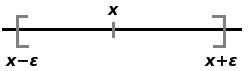
\includegraphics[scale=0.8]{Interval.png} \end{center}
    
    The goal of this method is to give the percentage of certainty which allows to obtain reliable and robust results. In tow dimensions, intervals are represented by boxes. Here is an example of the resolution by Intervals. It is the result of S1|S2 with:
    
    	\vspace{0.6 cm}
    	

    \begin{center} 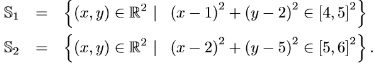
\includegraphics{Formule1.png} \end{center}
    
    \begin{figure}[!h] 
    \center
    	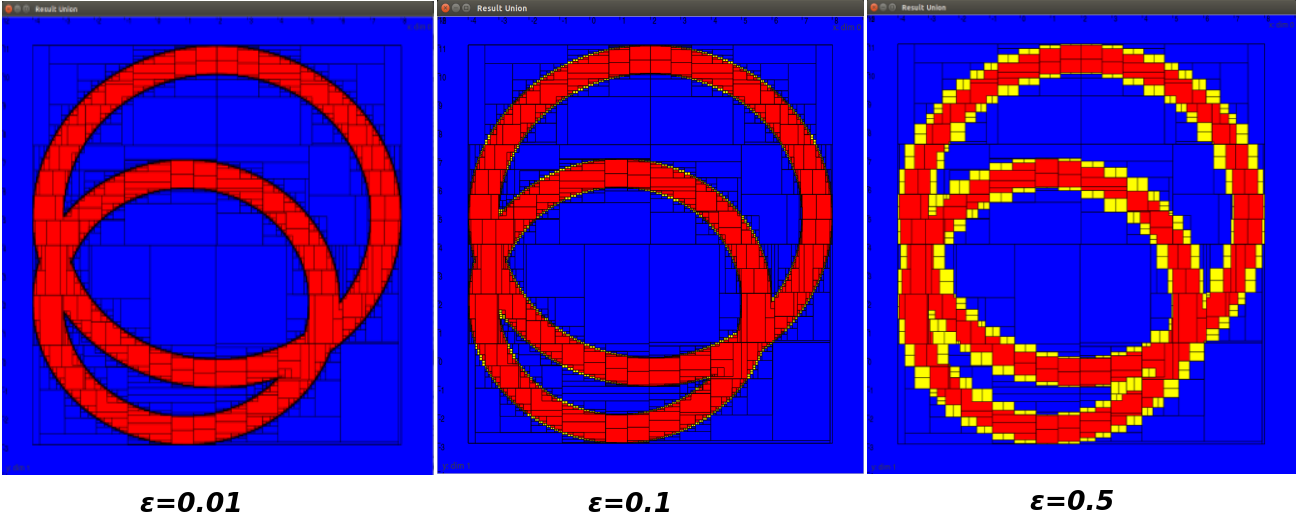
\includegraphics[scale=0.4]{Boxes.png} 
    	\caption{Resolution of S1 U S2 for different precision with intervals calculation } 
    \label{S1 U S2}
	\end{figure} 

	\newpage

	If a box frames a solution, it is cut in two parts and the calculation is reiterated on these two boxes which allow to discriminate one of them and to reduce solutions. However, this operation take lot of time because the number of boxes increase of  2n each time. That is why, the contractors are used, they allow to refine the boxes at the intervals which include strictly the solution before to cut them. This method allow to have an important gain of time during the simulation. 

	\begin{figure}[!h] 
    \center
    	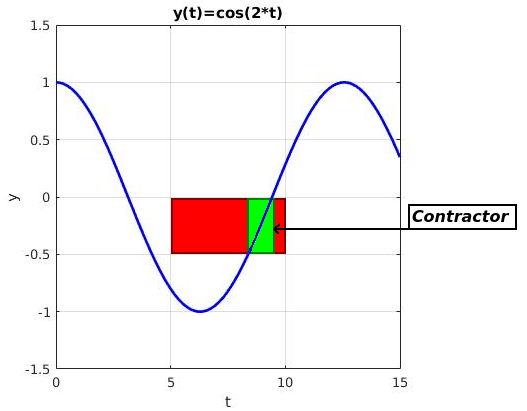
\includegraphics[scale=0.8]{Contractor.png} 
    	\caption{Example of the utilisation of contractor} 
    \label{Contractor}
	\end{figure} 
	
	For the example, the signal cos(2*t) in blue is used. The box in red corresponds to the normal box and the green box corresponds to the contractor. With this example, we can easily see that contractors improve  the simulation in terms of time. 

	\vspace{0.5 cm}
	
	For the simulation of the Gascogne project, we used a SIVIA function which make the paving for the representation of the France, robots control and their erosion.
	
	
\end{document}

